% !TEX encoding = UTF-8 Unicode

\documentclass[12pt,reqno]{amsart}
\usepackage[russian]{babel}
\usepackage[utf8]{inputenc}
%\usepackage[dvips]{graphicx,graphics}
\usepackage{graphicx}
\usepackage{euscript}
\usepackage{graphics}
%\usepackage{russcorr}
\usepackage[active]{srcltx} % SRC Specials: DVI [Inverse] Search
\usepackage{amssymb,amsmath,amsthm,amsfonts}
\usepackage{amsopn}
\newtheorem{cor}{Следствие}
\newtheorem{lem}{Лемма}
\newtheorem{thm}{Теорема}
\newtheorem{prop}{Предложение}
\newtheorem*{thm_pres}{Теорема}
\theoremstyle{definition}
\newtheorem{defn}{Определение}
\newtheorem{defneq}{Эквивалентное определение}
\theoremstyle{remark}
\newtheorem*{rem}{Замечание}
\newtheorem*{deff}{Обозначение} 
\usepackage{verbatim}
\usepackage{listings}
\usepackage{hyperref}
\usepackage{color}

\definecolor{dkgreen}{rgb}{0,0.6,0}
\definecolor{gray}{rgb}{0.5,0.5,0.5}
\definecolor{mauve}{rgb}{0.58,0,0.82}

\lstset{frame=tb,
  language=Java,
  aboveskip=3mm,
  belowskip=3mm,
  showstringspaces=false,
  columns=flexible,
  basicstyle={\small\ttfamily},
  numbers=none,
  numberstyle=\tiny\color{gray},
  keywordstyle=\color{blue},
  commentstyle=\color{dkgreen},
  stringstyle=\color{mauve},
  breaklines=true,
  breakatwhitespace=true,
  tabsize=3
}

\newcommand{\sug}[1]{\rule[-2mm]{0.4pt}{5mm}_{\,{#1}}}
\newcommand{\gen} {$GE^+_n(\mathbf{R}[x])\ $}
\newcommand{\genn} {$GE^+_2(\mathbf{R}[x])\ $}
\newcommand{\gn} {$G_n(\mathbf{R})\ $}
\newcommand{\gln} {$GL_n(\mathbf{R}[x])\ $}
\newcommand{\p} {\mathbf{P}}
\newcommand{\peq} {$\mathcal{P}$}
\newcommand{\po} {$\mathcal{P}_0$}
\newcommand{\ff} {$\mathbf{R}\ $}
\newcommand{\fx} {\mathbf{R}[x]}
\newcommand{\fp} {\mathbf{R_+}}
\newcommand{\fxp} {\mathbf{R_+}[x]}
\newcommand{\zx} {\mathbb{Z}[x]}
\newcommand{\zxp} {\mathbb{Z_+}[x]}
\newcommand{\basering} {$\mathbf{F}$}
\newcommand{\lfrac} [2] {\displaystyle \frac{#1}{#2}}
\newcommand{\brsum} [3] {\displaystyle \sum \limits_{#1}^{#2} \left( #3\right)}
\newcommand{\lsum} [2] {\displaystyle \sum \limits_{#1}^{#2}}
\newcommand{\br} [1] {\left( #1 \right)}
\newcommand{\tab} {\mbox{             } \quad }
\usepackage{a4wide}
\begin{document}

\begin{center}
\Large{\bf Отчет по домашней работе.}

\end{center}

\section{Постановка задачи}


В данной необходимо решить задачу классифицирования вида цветка ириса (Iris-Setosa, Iris-Versicolour, Iris-Virginica) по следующим признакам -- длина чашелистиков, ширина чaшеристиков, длина лепестка и ширина лепестка, посредствам использования нейронной сети.

\subsection{Данные}


Данный датасет можно найти в питоновской библиотеке -- sklearn.datasets с помощью функции load\_iris. Датасет состоит за 150, по 50 на каждый из трех типов цветка, каждый пример -- массив из четырех чисел и ответ — число от 0 до 2.

\begin{lstlisting}
from sklearn                     import datasets

orig_data = datasets.load_iris()
target = orig_data.target
data   = orig_data.data
\end{lstlisting}

Визуализируем данные:

\begin{lstlisting}
import matplotlib.pyplot as plt
from sklearn import datasets

iris = datasets.load_iris()
X = iris.data[:, :3]
Y = iris.target

x_min, x_max = X[:, 0].min() - .5, X[:, 0].max() + .5
y_min, y_max = X[:, 1].min() - .5, X[:, 1].max() + .5

plt.figure(2, figsize=(8, 6))
plt.clf()

plt.scatter(X[:, 0], X[:, 1], c=Y + 1)
plt.xlabel('Sepal length')
plt.ylabel('Sepal width')

plt.xlim(x_min, x_max)
plt.ylim(y_min, y_max)
plt.xticks(())
plt.yticks(())

plt.show()
\end{lstlisting}

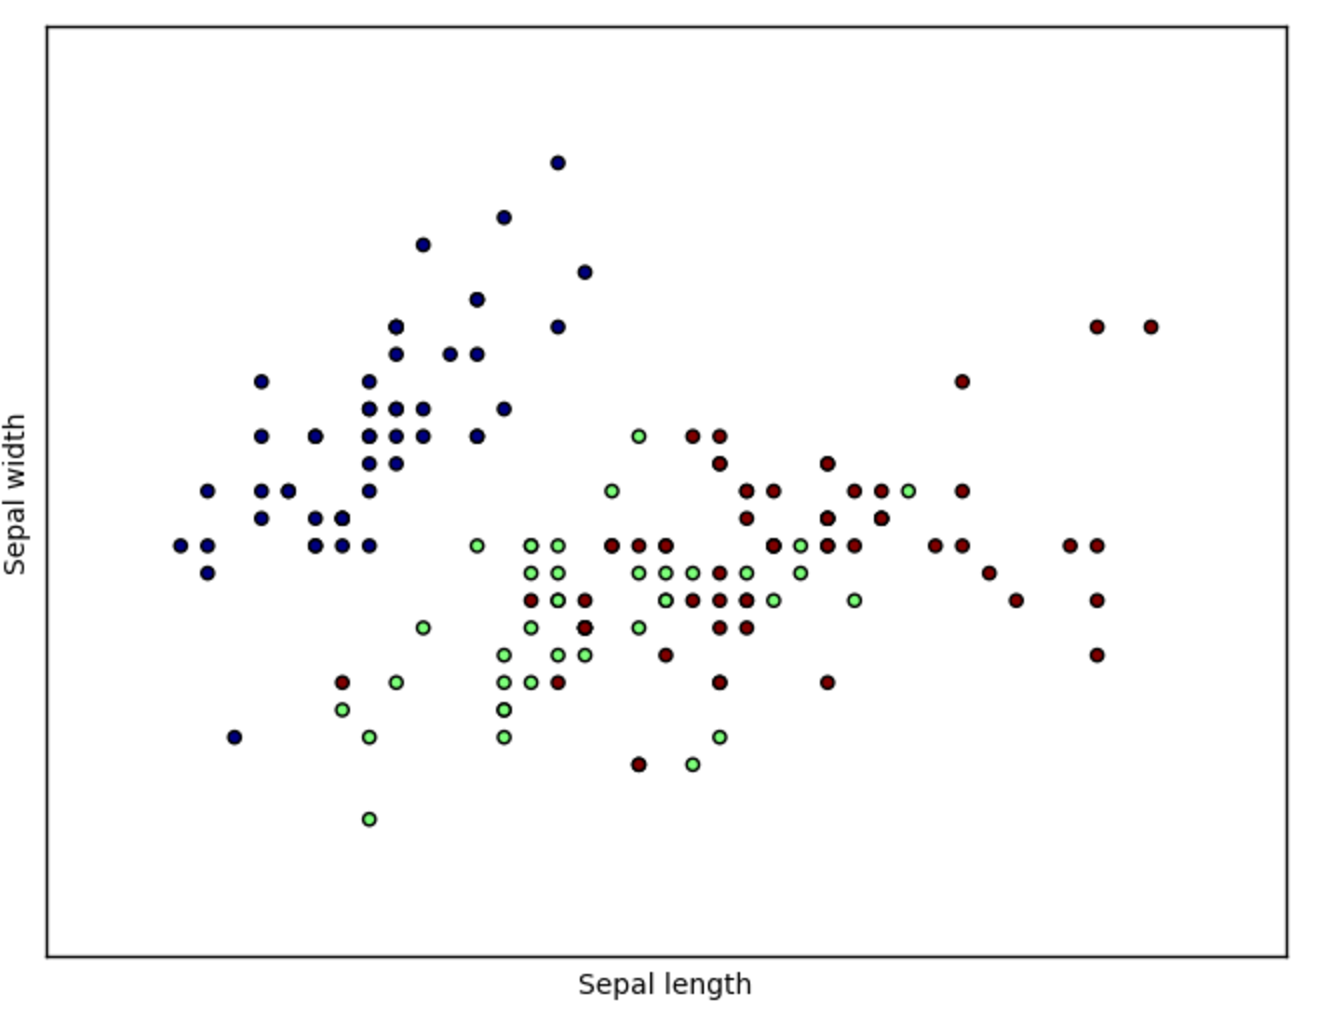
\includegraphics[width=0.9 \textwidth]{2.png}


\begin{lstlisting}
import matplotlib.pyplot as plt
from sklearn import datasets

iris = datasets.load_iris()
X = iris.data[:, 2:]
Y = iris.target

x_min, x_max = X[:, 0].min() - .5, X[:, 0].max() + .5
y_min, y_max = X[:, 1].min() - .5, X[:, 1].max() + .5

plt.figure(2, figsize=(8, 6))
plt.clf()

plt.scatter(X[:, 0], X[:, 1], c=Y + 1)
plt.xlabel('Petal length')
plt.ylabel('Petal width')

plt.xlim(x_min, x_max)
plt.ylim(y_min, y_max)
plt.xticks(())
plt.yticks(())

plt.show()
\end{lstlisting}

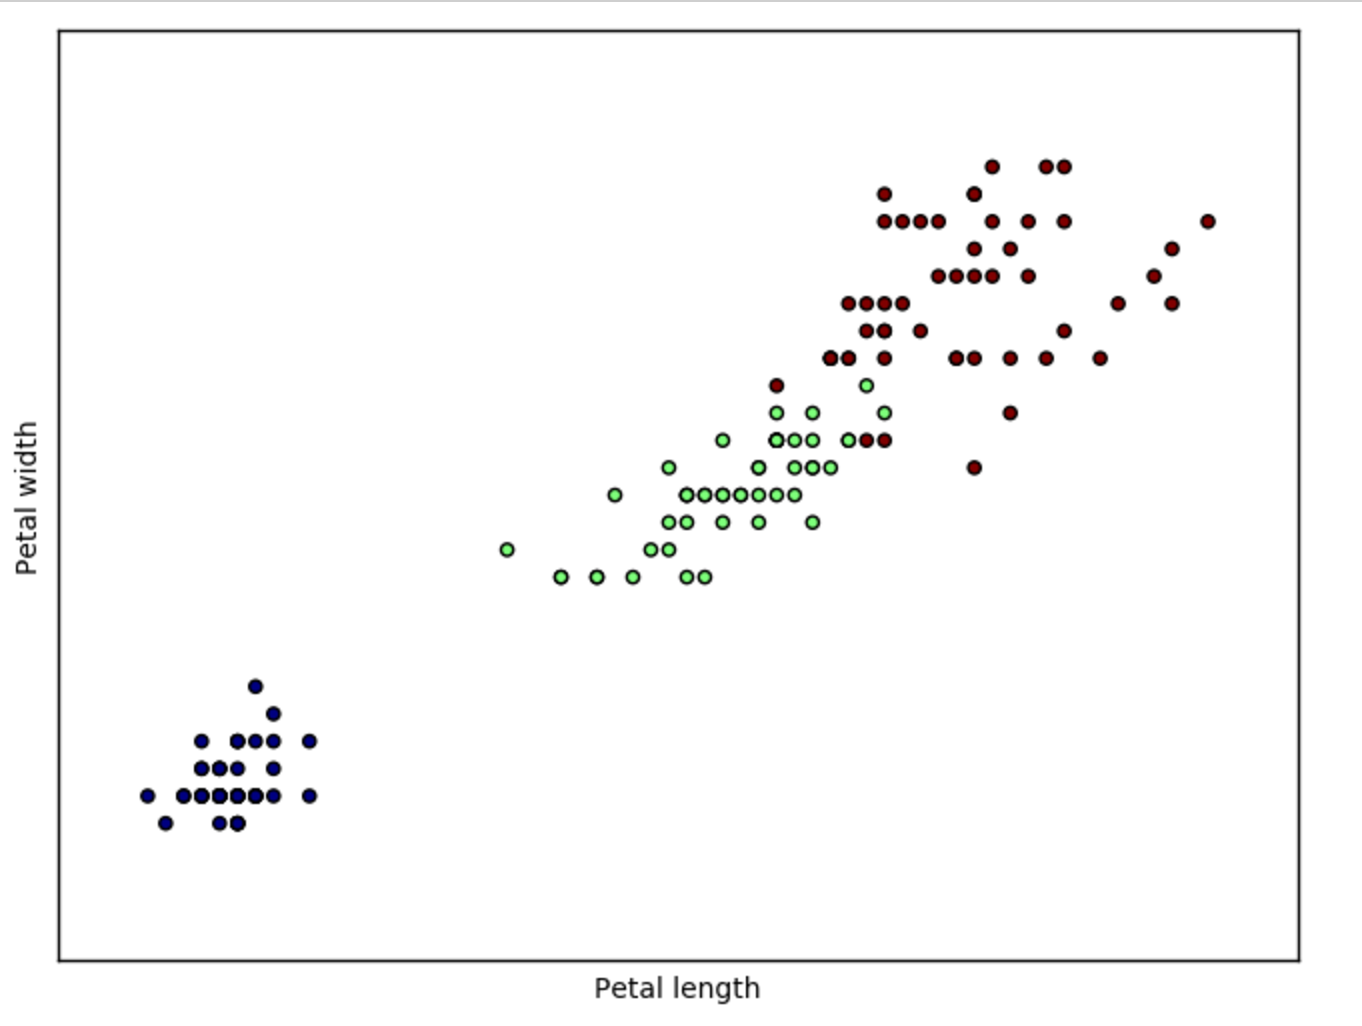
\includegraphics[width=0.9 \textwidth]{3.png}

Видно что по некоторым параметрам ответы датасета линейно разделимы -- значит нам хватит сети с одним скрытым слоем и не обязательно делать ее сильно нелинейной.

\section{Решение задачи}

\subsection{Нейронная сеть}


Для решения задачи было решено использовать библиотеку pybrain. В качестве нейронной сети была выбрана feedforward neural network (сеть прямого распространения сигнала) с одним полносвязным скрытым слоем.
\begin{lstlisting}
from pybrain.datasets            import ClassificationDataSet
from pybrain.tools.shortcuts     import buildNetwork
from pybrain.supervised.trainers import BackpropTrainer
from pybrain.structure.modules   import SoftmaxLayer
from pybrain.structure.modules   import LinearLayer
from pybrain.structure.modules   import SigmoidLayer
from pybrain.structure           import FullConnection

from sklearn.cross_validation    import train_test_split

from sklearn.model_selection     import cross_val_score
from sklearn                     import datasets

import matplotlib.pyplot as plt
import numpy             as np
import pandas            as pd

def convert_supervised_to_classification(data, target):
    num_tr = data.shape[0]

    traindata = ClassificationDataSet(4,1,nb_classes=3)
    for i in range(num_tr):
        traindata.addSample(data[i], target[i])

    traindata._convertToOneOfMany()
    return traindata

def net_model_pybrain():
    network = FeedForwardNetwork()
    inLayer = LinearLayer(4)
    hiddenLayer = SigmoidLayer(1)
    outLayer = SigmoidLayer(3)

    network.addInputModule(inLayer)
    network.addModule(hiddenLayer)
    network.addOutputModule(outLayer)

    in_to_hidden = FullConnection(inLayer , hiddenLayer)
    hidden_to_out = FullConnection(hiddenLayer , outLayer)

    network.addConnection(in_to_hidden)
    network.addConnection(hidden_to_out)

    network.sortModules()
\end{lstlisting}

\subsection{Обучение сети}


Для начала создадим сеть

\begin{lstlisting}
traindata = convert_supervised_to_classification(data, target)
network = buildNetwork(4,1,3,outclass=SoftmaxLayer)
trainer = BackpropTrainer(network, dataset=traindata, momentum=0.1, verbose=True)
\end{lstlisting}

Далее обучим ее на наших данных на 100 эпохах и построим график ошибки.

\begin{lstlisting}
epochs = 100

from matplotlib import pyplot as plt
%matplotlib inline


x = []
y = []
for i in range(epochs):
    x += [i]
    y += [trainer.train()]

plt.plot(x, y)
\end{lstlisting}

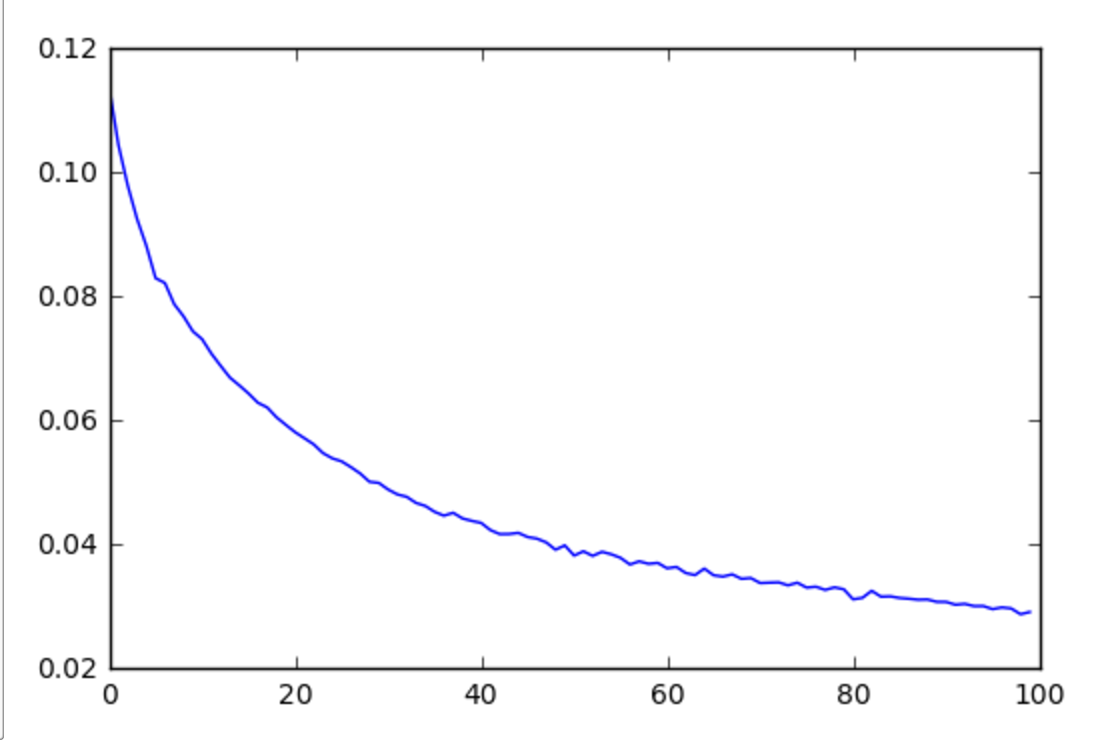
\includegraphics[width=0.9 \textwidth]{1.png}

Из графика видно, что ошибка нейронной сети на данном датасете оказалась, в конченом итоге, достаточно мала, учитывая, что данных было не так уж и много. Так же под конец ошибка начинает стабилизироваться, что говорит о том что алгоритму требуется не так уж и много эпох что бы придти к оптимальной модели.
\end{document}
